%! TEX root = diss.tex
\documentclass[../diss.tex]{subfiles}
\chapter{Evaluation}

In this chapter, I review the software produced in the implementation phase.
I relate systems and algorithms built to the success criteria in the project
proposal, and describe how the work done exceeds what I initially set out to do.
This is done by looking at the \ac{MatSquare} algorithm, the parallel system
simulated, and the optimisations applied.
I review the tests I conducted to assert correctness. Then I proceed to
discuss the advantage of parallel computation for solving \ac{APSP}, where
I demonstrate that the benefit is large, even for different types of parallel
computers.


% TODO: intro to three types of computer, then write something about Cal,
%   possibly limits to evaluation as would expect linear decrease and higher
%   efficeincy for the earlier ones looking at the trends

% ** Other points **
% All unit tests passed (screenshot)
% Some points to show:
% * Exploits parallelism for simulation (was close to 800% CPU usage when `htop`)
% * Very expressive interface, and also raised exceptions like ..., when misused,
%   made development of parallel algorithm a lot easier
% * Extension: Generalized FoxOtto, ran on the same tests, and still produce
%   correct results (unit tests again)
% * Extension: MIMD timing simulation, unit tests
% * Extension: Graph compression, also not just mapped queries to reduced graph and give
%     path length, but also reconstruct list of nodes in original graph.
%     Reference figure as an example
% * Paragraph discussing main plot... TODO: what to say about this?
% * The whole thing about mapping onto real-hardware to do sensitivity analysis
% * Asymptotic complexity of algorithm

% Parallel MatSquare:
% * This section should cover the first 3 points above, quoting them as well...
% * Can have subsections as appropirate
% * squeeze in graph compression somewhere here?
% Parallel MatSquare {{{
\section{Parallel MatSquare}%
\label{sec:Parallel MatSquare}

\begin{wrapfigure}{r}{0.5\textwidth}
    \vspace{-25pt}
    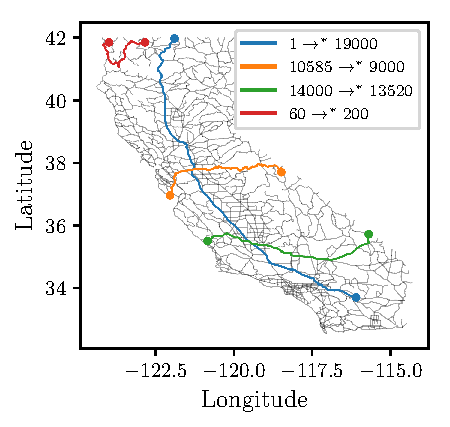
\includegraphics[scale=1]{figs/cal-node-paths.pdf}
    \caption[Four example shortest-paths in the Californian road network]{Four example shortest-paths in the Californian road network
        ($|V|=21048$, $|E|=21693$). These paths consist of
        575, 328, 272, and 207 nodes, respectively.
        % TODO next: Git commits, explain that make diagram, add all diagrams
        %    to GitHub as backup.
    }%
    \label{fig:cal-node-paths}%
    \vspace{-55pt}
\end{wrapfigure}

% (1) MatMul-based algo, find shortet path, can give list of nodes
%  * Manualled created resulted for some set of example graphs (see appendix)
%  * Also implemented serial dijkstra routine that is simple to prove
%    correctness of, and compared the result on $362^2$ possible pair paths on a
%    random large graph, as a unit test. Gives same results
%  * Show example list of nodes, and can make a simple plot on the California
%    road network, on compressed graph, showing a long path...
I successfully implemented the \ac{MatSquare} algorithm. 
I initially set out to
``\textit{[implement] an algorithm based on matrix multiplication that can find
the length of the shortest path between all pairs of nodes in a graph, and it
is able to give the list of nodes that make up such paths.}'' This resulted in
the \ac{MatSquare} algorithm, which is indeed based on matrix multiplication,
as shown in lines 7--8 in \cref{alg:matsquare}. I also completed the extension
to generalise \ac{MatSquare}, such that it could solve a problem of size $n$
with a different \ac{PE} grid-size $p \neq n$, both smaller and larger.
To assert the correctness of the
path lengths and the path reconstruction, I manually computed the results for
two small graphs, then compared it with the algorithm's output.  Additionally,
I took a subsection of one of the real-world graph datasets\footnote{I used
    as script to extract all the vertices and edges
    within a fixed distance of a point in the centre of the city of
Oldenburg. This gave a graph with 430 nodes and 476
edges. See \cref{sec:extract} for more details.}, and tested the path lengths and reconstructions on all $|V|^2$ pairs.
To do this, I implemented Dijkstra's algorithm with path-reconstruction, which
is a easier to prove the correctness of compared to the \ac{MatSquare}
algorithm. I then ran this and my algorithm and asserted the equality of the
results for all $430^2$ vertex-pairs. We can see the results of these tests in
\texttt{MatSquareTest} in \cref{fig:unit-test}. This was  done for
both the regular and generalised version of the algorithm.

\begin{wrapfigure}{r}{0.47\textwidth}
\begin{center}
    \vspace{-15pt}
    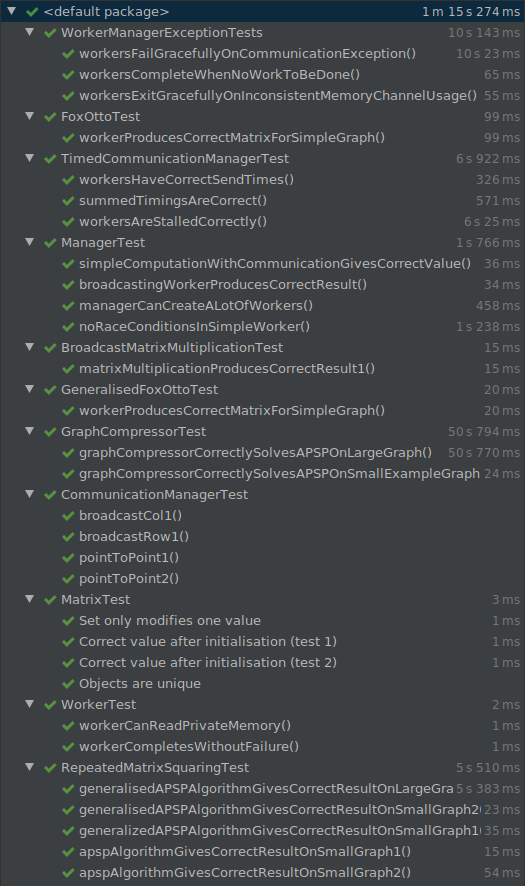
\includegraphics[scale=.4]{figs/unit-test-success.png}
\end{center}
\caption[Screenshot of unit tests passing]{A screenshot showing all the unit tests written and that they passed.}
\label{fig:unit-test}
\vspace{-10pt}
\end{wrapfigure}

I also successfully extended the project with the graph compression optimisation.
Arbitrary undirected graphs can be compressed through removal of two-degree nodes,
which I have tested by comparing the output to manually-compressed graphs for
adversarially chosen example graphs.
The algorithm for mapping \ac{APSP} queries to the compressed
graphs and mapping the results back is also correct. I verified this by
comparing the paths found when compressing the graph to the output from
\ac{MatSquare} running on the same graph, but uncompressed. I did this in a unit
test in \cref{fig:unit-test}, and found that it could correctly reconstruct the
list of vertices in all $430^2$ paths in a large graph.
To further
demonstrate that paths are reconstructed properly when mapping results from
the compressed graph to the uncompressed one, I ran four example queries on the
Californian road network and plotted the list of vertices returned in
\cref{fig:cal-node-paths}, using additional data about each vertex's
geographical position. Solving \ac{APSP} on such a large graph would be
infeasible to do quickly without the graph compression optimisation.

% (3) Routine minimises amount of data movement
%  * FoxOtto technique is used,
%  * Looking at code, we only send over a single interconnect, so all the data
%    is in the right location after moving it only once. This is clearly
%    minimal if we do not have shared memory. Additionally, no congested
%    interconnect as this would throw `....`
%  (? Table with counts for the number of memory movements in total? ?)
I set out to ``\textit{... minimise the amount of data movement between
processing elements, which is done by using techniques such as Fox-Otto's
algorithm}'' in the matrix-multiplication routine of the \ac{MatSquare}
algorithm. The data movement pattern used is based on the technique
\citeauthor{fox} used \cite{fox}. As we see in \cref{alg:foxOtto}, this makes all the
\acp{PE} have exactly the data that they need at each computation phase, after
sending a message across a single interconnect channel and possibly an uncontested
row-broadcast channel as well. This is clearly minimal data movement if
we are not allowed to utilize shared memory and each \ac{PE} cannot have more
than $O(\lceil n^2 / p ^2 \rceil)$ private memory.

% }}}

% Parallel simulation:
% (2) MatMul routine parallelised, runs on parallel simulation,
%     each PE can send data
%  * Unit tests for this interface, first show interface working
%  * Show `FoxOtto`, `GeneralisedFoxOtto` and corresponding unit tests
%  * Further evidence of correctness is correctness test for paths, The paths
%    found are unlikely to be correct if the matrix mult. routine is faulty
% * Point on parallelism worked well, 800% CPU
% * Turned out very expressive, and useful exception reported back
% Parallel simulation {{{
\section{Parallel simulation}%
\label{sec:Parallel simulation}

The parallel simulator met all the requirements laid out in
\autoref{sec:Requirements analysis}, which resulted in ``... \textit{a simulated
massively parallel processor, where each processing element can send data to
each other through simulated interconnects.}'' When creating the
\texttt{Manager} and \texttt{TimedManager}, I can configure the number of
\acp{PE} and the interconnect topology, respectively. The \texttt{Worker}
interface for writing parallel programs is simple to use, but has expressive
power beyond what I required. It also cleanly threw useful exceptions such as
\texttt{InconsistentCommunicationChannelUsageException} if the programmer did
not correctly match up \texttt{send}s and \texttt{receive}s. The
interface and its capability has been thoroughly tested through unit
tests that cover usage much
more complex than the what was needed by \cref{alg:foxOtto}. The computation
time measures  reduce the amount of noise, which gives better measurements.
Additionally, a \ac{MIMD} model is used for the communication time, which is more
complicated to implement compared to the proposed na{\"i}ve \ac{SIMD} model, but with
the benefit of giving a more realistic simulation. Lastly, the simulator runs in
parallel by simultaneously executing worker-phases. This sped up
simulation a lot, as computing the results for the compressed Californian road
network for instance took about 25 minutes and the \ac{CPU}
usage was close to 800\% while doing so\footnote{%
I measured this using \texttt{htop}},
which shows that the parallelisation was successful in practice.
% TODO: this last sentence a bit fluffy, maybe compared with Serial Dijkstra time
%       ot compute, but in that case would need disclaimer on not built for my
%       system

I also successfully ``\textit{[p]arallelised the matrix multiplication routine
of the [\ac{MatSquare}] algorithm to run on [the parallel system simulator]}''.
This was achieved with the  \texttt{FoxOtto} and
\texttt{GeneralisedFoxOtto} classes,
which use the \texttt{Worker} interface to create
a parallel algorithm where coordination happens through message passing. The
\texttt{Manager} allows intermediate results from each \ac{PE} to be fetched
after each phase, which I used in my unit tests to verify that the distance
product was computed correctly on test matrix inputs. Another justification for
the correctness of the parallel matrix multiplication step is the \ac{MatSquare}
unit tests. For these, I used the parallel matrix multiplication step instead
of a serial one, and it is unlikely for the shortest paths to be correct if there
are any faults in the parallel distance product subroutine.

% }}}

% Advantage of parallel computation for solving APSP
% (4) High parallel efficiency for solving APSP
%  * Refer back to equation 2.3 in section 2.1 about computation ratio, then
%    refer to the computation ratio plots and say that high parallel efficeincy,
%    above 90% when problem suffcienctly sub-divided
% * Discuss the main plot, and explain sensitivity analysis
% * Explain the first column of plots as well...
% Advantage of parallel computation for solving APSP {{{
\section{MatSquare timing measurements}%
\label{sec:MatSquare timing measurements}

Recalling the aim laid out in \cref{sub:Related work}
we want to evaluate the benefit of parallel computation on
a wide range of parallel systems. With this purpose, I justify my choice of
communication parameters. Then I plot and discuss their effect on both
the total execution time and the parallel efficiency achieved on a wide
range of input graphs with real-world characteristics.

\begin{figure}
    \centering
    \subfigure[Multi-core processor (Sandy Bridge)]{%
        \label{fig:main-plot-fig-a}%
        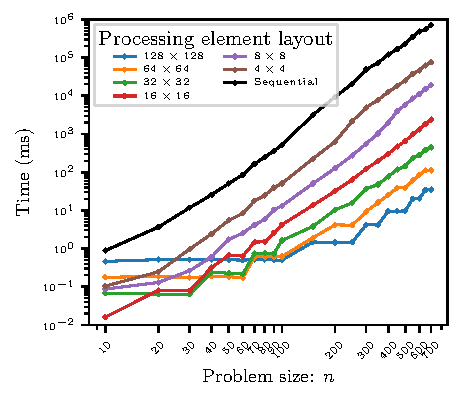
\includegraphics{figs/plots/total-time-scaling-sandy-full-width-no-errorbars.pdf}%
        \hfill%
        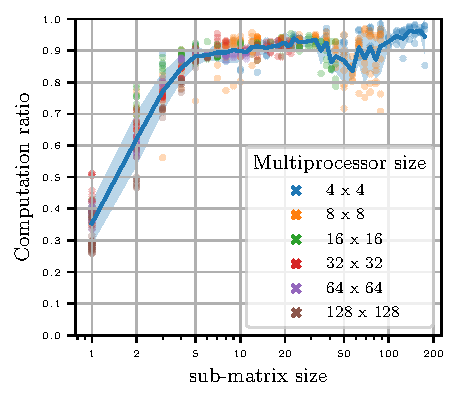
\includegraphics{figs/plots/ratio-bucket-sandy-half-scale.pdf}
    }%
    \vskip\baselineskip\vspace{-25pt}%
    \subfigure[Supercomputer (Sunway  TaihuLight)]{%
        \label{fig:main-plot-fig-b}%
        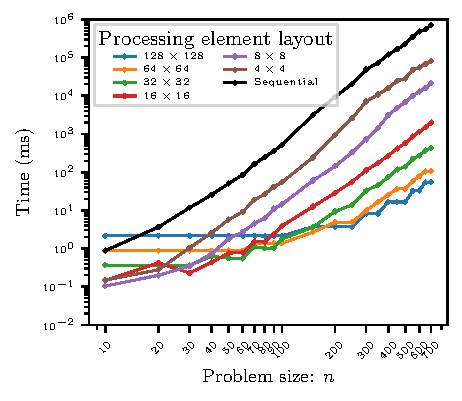
\includegraphics{figs/plots/total-time-scaling-taihu-full-width-no-errorbars.pdf}%
        \hfill%
        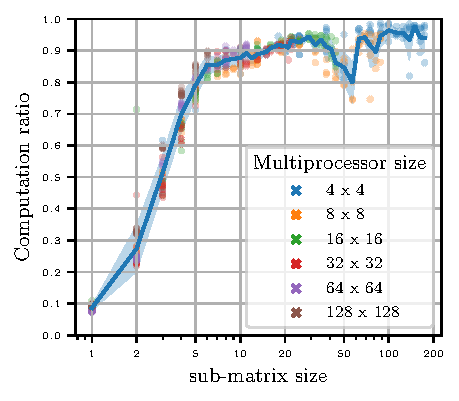
\includegraphics{figs/plots/ratio-bucket-taihu-half-scale.pdf}
    }%
    \vskip\baselineskip\vspace{-25pt}%
    \subfigure[Distributed computer (Internet)]{%
        \label{fig:main-plot-fig-c}%
        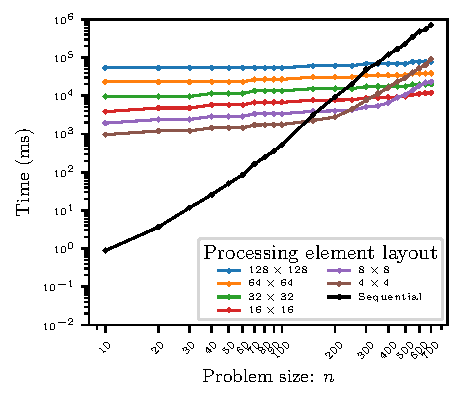
\includegraphics{figs/plots/total-time-scaling-internet-full-width-no-errorbars.pdf}%
        \hfill%
        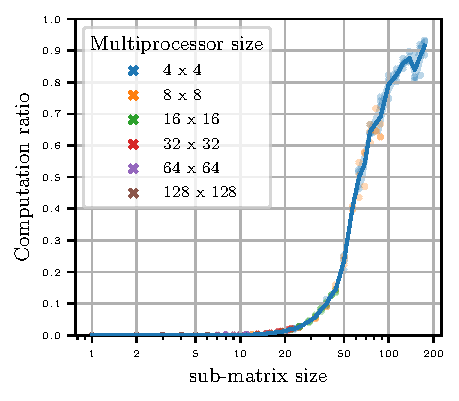
\includegraphics{figs/plots/ratio-bucket-internet-half-scale.pdf}
    }%
    \caption[Plot of execution time scaling and computation ratio for the MatSquare algorithm on three different parallel systems]{To the left, the total execution time of \ac{MatSquare} is
        plotted for different graphs with $n=|V|$ vertices.  To the right, I
        group computation ratios by the size of the sub-matrix each \ac{PE} is
        responsible for.  Confidence intervals are omitted from the left plots
        because they are mostly negligible, but can be found in
    \autoref{sec:Error bars} in the appendix.}
    \label{fig:main-eval-plot}
\end{figure}

% TODO: Introduction tying this section's subs together
% Choice of communication parameters:
% * sensitivity analysis
% * map onto real hardware for more applicable conclusions
% * The three models used and reference
\subsection{Choice of communication parameters}%
\label{sub:Choice of communication parameters}

By basing the communication constants on real hardware, we can draw more
applicable conclusions. For the parallel system simulator to estimate the
message-passing delay, we must specify the latency and bandwidth. As we reviewed
in \autoref{sec:Parallel computing}, there are many classes of parallel computers,
ranging from multi-core processors to different computers communicating over the
Internet. To get a sense of what the benefit of parallelism is across
this whole range,
I consider the two extremes and a supercomputer that lies in-between.
For each class, I base the communication constants of a
real-life system within the class. The values chosen are summarised in
\cref{tab:communication-constants}.

% Sandy bridge
\paragraph{Multi-core processor}%
\label{par:Multi-core processor}

The Sandy Bridge microarchitecture supports multiple cores which execute in
\ac{MIMD} fashion, and the L3 cache is shared across all cores while the
lower-level caches are local to each core \cite{sandyBridge}. For one core to
send data from its private L1 cache to another core's L1 cache, we must look
at the round-trip time of the cache coherence protocol because the receiving
core must message the sending core and wait for the cache line to
come back. \citeauthor{timJones} have measured the latency of this,
and found that for the Sandy Bridge microarchitecture, the
round-trip latency is about 107 clock cyles
80\% of the time \cite{timJones}. I make the simplifying
assumption that the latency is always 107 cycles, and the latency is
independent of the processor's clock frequency. 
The ring interconnect, used to implement
cache coherency in the Sandy Bridge microarchitecture, has a
bandwidth of 32 bytes per cycle. I will assume this is is the available
bandwidth for message-passing.

% Cite these guys: \cite{sandyBridge} and \cite{timJones}.

% Taihu light
\paragraph{Supercomputer}%
\label{par:Supercomputer}

For the supercomputer parallel system, I have based by constants on the
Sunway TaihuLight system, which consists of several SW26010 processors
connected together through a system interface with a bidirectional bandwidth
of 16~GB/s and a latency around 1~{\textmu}s \cite{sunway}. Each SW26010 processor
consists of 256 computer processing elements which can themselves communicate
with lower latency and higher bandwidth, and they also run at a lower clock
frequency than that of my laptop. I do not simulate this memory hierarchy, 
but instead assume that each individual \ac{PE} is connected
through the system interface used on the Sunway TaihuLight system, and executes
instructions at the same clock frequency as my laptop. I also half the bandwidth
because messages-passing is one-directional in the architecture assumptions
laid out in \cref{sec:Parallel architecture assumptions}.

\paragraph{Distributed computer}%
\label{par:Distributed computer}

For this parallel system, I am assuming that we have some set of \acp{PE} that
are distributed geographically across Europe, and they communicate by sending
packets over the Internet. This kind of system is very scalable as it is easy
to add new \acp{PE}, but we expect the communication constants to be higher.
Within Europe, ICMP packets have been measured to have an average
round-trip time latency of under 15~ms, but I use a generous upper-bound
of 30~ms because other continents might have higher latencies \citep{verizon}.
I also use the round-trip time to allow  communication to happen with protocols
where acknowledgement messages are sent as well, such as TCP.
For the bandwidth, I used the regional average broadband speed across
Western Europe, which is 90.56~Mbps \cite{broadband}.

\begin{table}
    \centering
    \begin{tabular}{|c|c|c|}
        \hline
        \textbf{Parallel system} & \textbf{Latency} & \textbf{Bandwidth} \\
        \hline
        Multi-core processor & 107 clock cycles\footnotemark & 32 Bytes per
        cycle\footnotemark \\
        \hline
        Supercomputer & 1~{\textmu}s & 8~GB/s \\
        \hline
        Distributed computer & 30~ms & 11.25~MB/s \\
        \hline
    \end{tabular}%
    \caption[The communication constants used in evaluation]{The communication constants used in my timing analysis of the
    \ac{MatSquare} algorithm. Note that for small submatrix-sizes $n'$, the
    latency will be the dominating contributor
    to the message-passing cost, not the bandwidth.}%
    \label{tab:communication-constants}%
\end{table}

\footnotetext[2]{With the clock frequency of my system, this corresponds to
46.52~ns}
\footnotetext{With the clock frequency of my system, this corresponds to
68.55~GB/s}

% Discuss total time scaling
% * As num. PE *4, we have a decrease in computation time, decrease gets slightly
%   smaller the more low we go, this is for large problem sizes where even out
% * At the start, there are many flat lines, with stepwise increase, this is
%   because of asymptotic complexity, and padding requiered
% * As increase communication constants, serial gets better, but parallel always
%   catches up eventually,

% Discuss parallel efficiency
% * Related parallel computation to efficiency
% * quote success criteria
% * show that for all parameter choices, evenually reach over 90 and even 95\%
%   efficiency
\subsection{Advantage of parallel computation for solving APSP}%
\label{sub: of parallel computation for solving APSP}

\begin{figure}[t]
    \centering
    \subfigure[Total time]{%
        \label{fig:california-total-time}%
        \centering%
        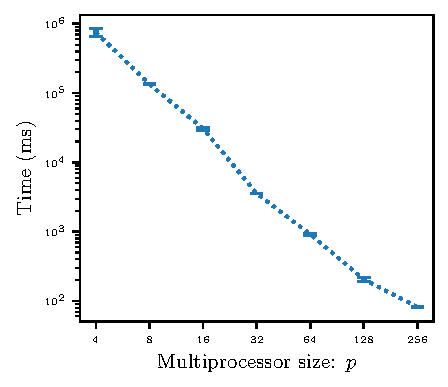
\includegraphics[scale=1]{figs/plots/total-time-california.pdf}%
        }%
    \subfigure[Computation ratio]{%
        \label{fig:california-ratio}%
        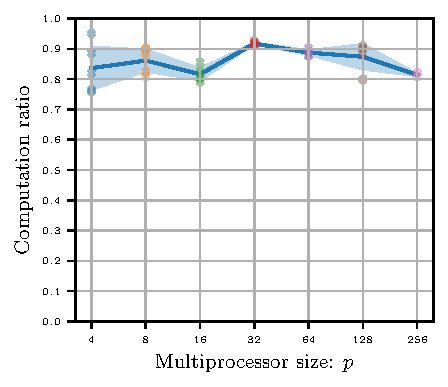
\includegraphics[scale=1]{figs/plots/bucket-california.pdf}%
    }%
    \caption[Execution time and computation ratio of MatSquare on the Californian road network]{Execution time measurements and computation ratio achieved
    when running \ac{MatSquare} on the compressed Californian road network ($|V|=1408$). I used communication constants based on a multi-core processor (Sandy Bridge).}%
    \label{fig:california-plot}
\end{figure}

In \cref{fig:main-eval-plot}, we see the scaling of the total execution time
and the computation ratio when running \ac{MatSquare} on different problem
sizes. I start this subsection
by discussing the general trends in the total time scaling in
figures \ref{fig:main-plot-fig-a} and \ref{fig:main-plot-fig-b}. Then I relate the plots
to the parallel efficiency, and demonstrate the final success criteria while
discussing the benefit of parallel computation on different machines and
problem sizes.

For the multi-core and supercomputer configuration,
the total execution time does not increase, or increases step-wise,
 for small problem sizes. This is especially noticeable for large \ac{PE} layouts.
In the flat portions, we have
enough \acp{PE} for each cell in the input matrix, so increasing
the problem size does not cause more computation per \ac{PE}. The step-wise
increase  is caused by the input padding: To map for instance
a problem of size $n=200$ onto $64 \times 64$ \acp{PE}, we must pad the input
until the size is a multiple of 64, which can cause two different problem sizes
to be mapped to the same size, causing the same amount of computation to be performed.

As we get to larger problem sizes, the total times in figures
\ref{fig:main-plot-fig-a} and \ref{fig:main-plot-fig-b} start to even out
and approach linear in the log-log-scale. Comparing the trends for the different
values of $p$, we decrease the required computation time by a constant
factor whenever we multiply the number of \acp{PE} by 4. We also see this
for the compressed Californian road network in \cref{fig:california-total-time}.
This tells us that for
large problem sizes, there's always a benefit to adding more computation power
as this reduces execution time, even with a communication overhead.

We demonstrate the final success criteria by considering
the  parallel efficiency. As we saw in
\cref{eq:parallel-efficiency}, the parallel efficiency is equal to the
computation ratio. We can therefore think of the $y$-axis in three right-column
plots in \cref{fig:main-eval-plot} as measuring the parallel efficiency.  With
the multi-core processor and supercomputer configurations, we quickly achieve
$\varepsilon>0.9$ and it even reaches above 95\% eventually. This means the
\ac{MatSquare} algorithm is able to efficiently utilize the available
processing power on a parallel system without communication being a major
bottleneck.
The last success criteria is therefore achieved:
 ``\textit{The evaluation
of the algorithm demonstrates that parallel computation gives a high parallel
efficiency for solving APSP}''. We also see a parallel efficiency $\varepsilon > 0.8$
in \cref{fig:california-ratio}.

In figure \ref{fig:main-plot-fig-c}, we see that for a distributed computer,
there is little benefit to parallel computation compared with serial for
small problem sizes. When there are just a few {\textmu}s of computation
before we need to send a packet across Europe, there is a very large communication
overhead, which we see from the near-zero computation ratio for sub-matrices
of size less than 20. This is also why most of the execution time plots are flat,
since the communication is dominating. However, even with such a large
message-passing overhead,
we eventually achieve a high parallel efficiency, but this only happens
for the $4 \times 4$ and $8 \times 8$ arrangements for problem sizes where
$n \leq 700$. However, we can expect other arrangements to also get to this point
with larger problems. Also, as we reach the point where computation start to
dominate, the total execution time starts following a trend  similar to that
in figures \ref{fig:main-plot-fig-a} and \ref{fig:main-plot-fig-b}. Therefore,
we would expect the $128 \times 128$ configuration to overtake all the smaller
arrangements for some very large problem.

% }}}

% Summary
% Summary {{{
\section{Summary}%
\label{sec:Summary3}

In this chapter, I showed how the project met and exceeded the success criteria.
The parallel system simulator was showed to work well through unit tests, and
the interface it provides was very easy to work with. I demonstrated the
correctness of the main algorithm of the project and its generalised version.
Furthermore, I successfully asserted the correctness of the graph compression
optimisation by running it on demanding problem sizes. Lastly,
I looked at the timing measurements of \ac{MatSquare}
to prove the benefits of parallel computation for solving \ac{APSP} on
real-world-like graphs on a wide range of different parallel systems.

% The success criteria for creating parallel APSP algorithm and reconstructing
% paths was successfull, MatSquare. And I asserted its correctness with several
% unit tests
% Also successfully implemented graph compression optimisation, which has large
% gains in time-saving when executed on Californian road network.
% Also minimized the data movement.
%
% An efficient parallel simulation of a parallel system was implemented, and
% it provides an expressive interface to the programmer. Using this, I paralleised
% the MatSquare algorithm and tested it.
%
% Communication constants based on three three parallel systems of different
% types.
%
% Both the supercomputer and multi-core processors quickly achieve high parallel
% efficiency, meaning we benefit from parallel computation. For internet,
% takes a bit longer, but get same effect at this point

% }}}


% vim: foldmethod=marker
